\chapter{Provenance et contextes funéraires}\label{ch:provenance}

La provenance n’a pas partout la même résolution. « Rome », une voie, un cimetière, une région de catacombe, une tombe et un lieu de conservation correspondent à des informations différentes. Une référence aux ICUR permet un repérage bibliographique ; elle n’autorise pas à attribuer au monument tous les caractères du secteur couvert par le volume. Les notices de l’EDCS ne donnent que « Roma ». Les fiches de l’EDB précisent, pour la plupart des textes, le rattachement topographique retenu par les éditeurs (\emph{Pertinence}) et le lieu de conservation actuel. Ce chapitre exploite ces deux informations, sans les confondre et sans les traiter comme des données de fouille.

\section{Le volume des ICUR comme classement bibliographique}

Les \st{nC} textes funéraires se répartissent selon le volume des ICUR de leur première référence : \st{nVolI} relèvent du volume I, qui réunit les inscriptions dont la provenance s’est perdue ; 102 du volume IV (entre voies Appienne et Ardéatine) ; 94 du volume II (voies Cornelia, Aurelia, Portuensis et d’Ostie) ; 68 du volume III (voie Ardéatine) ; les autres volumes sont faiblement représentés, et 17 textes n’ont pas de référence ICUR. Cette structure reflète l’histoire de l’édition plus que celle des cimetières : le volume I réunit des inscriptions dispersées depuis le Moyen Âge, souvent transmises par des sylloges ou conservées dans des collections, et un grand nombre d’inscriptions datées.

\section{Le rattachement topographique selon l’EDB}

L’EDB attribue \st{nOrigInc} textes funéraires à la série d’origine incertaine et rattache les \st{nProvConnue} autres à un cimetière ou à un secteur (tableau~\ref{tab:cimetieres}, figure~\ref{fig:cimetieres}). Trois ensembles dominent : Calliste et ses aires à ciel ouvert, sur la via Appia ; Domitilla, avec la basilique des Saints-Nérée-et-Achillée, sur la via Ardeatina ; Commodilla, sur la via Ostiensis. Ils correspondent aux volumes IV, III et II des ICUR, dont ils précisent le contenu. Le rattachement de l’EDB ne coïncide pas toujours avec le volume : treize textes du volume I reçoivent de l’EDB un rattachement précis (Cyriaque, Pamphile, Saint-Valentin, Nicomède…), fruit des identifications postérieures à l’édition.

% généré par scripts/04_generated.py
\begin{table}[tbp]\centering\small\caption{Rattachement topographique des textes de l’ensemble C selon l’EDB (443 textes appariés). Les rattachements de moins de trois textes sont regroupés.}\label{tab:cimetieres}
\begin{tabular}{@{}l r@{}}\toprule Cimetière ou secteur & Textes\\\midrule
origine incertaine & 165 \\
Calliste (via Appia) & 70 \\
Domitilla (via Ardeatina) & 57 \\
Commodilla (via Ostiensis) & 40 \\
cimetière anonyme de la via Appia & 19 \\
cimetière anonyme de la via Ardeatina & 10 \\
entre via Appia et via Ardeatina & 8 \\
Saint-Pierre (Vatican) & 8 \\
Pontien (via Portuensis) & 8 \\
Cyriaque (via Tiburtina) & 6 \\
Octavilla / Saint-Pancrace (via Aurelia) & 5 \\
Saint-Paul (via Ostiensis) & 5 \\
aire de Lucine (via Appia) & 4 \\
Pamphile (via Salaria vetus) & 3 \\
Saint-Sébastien, ad Catacumbas (via Appia) & 3 \\
autres cimetières (Coem. Generosae) & 3 \\
autres cimetières (Coem. s.Theclae) & 3 \\
autres rattachements (moins de trois textes chacun) & 24 \\
\bottomrule\end{tabular}\end{table}


\begin{figure}[tbp]\centering
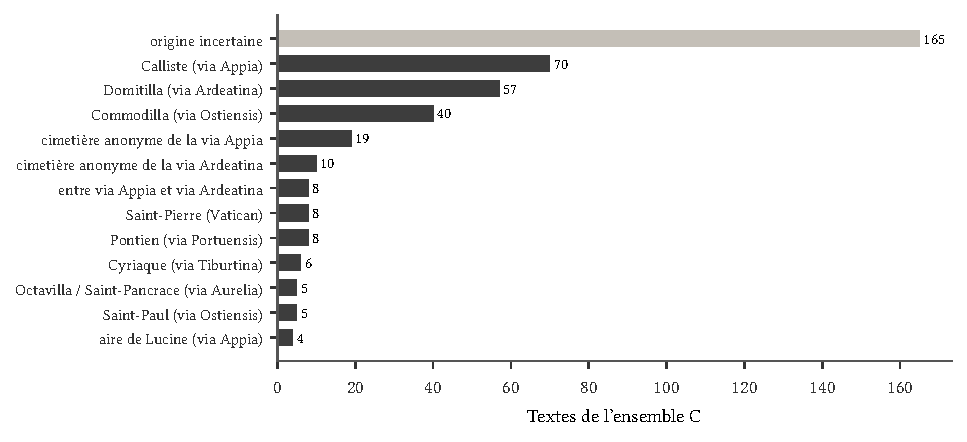
\includegraphics[width=0.88\linewidth]{figures/fig_cimetieres.pdf}
\caption{Rattachement topographique des textes funéraires selon l’EDB (secteurs d’au moins quatre textes).}\label{fig:cimetieres}
\end{figure}

La répartition par période des trois grands ensembles diffère. Les textes de Commodilla se concentrent dans les dernières décennies (1, 7, 13 et 19 textes pour les quatre périodes), alors que ceux de Calliste (7, 23, 19, 21) et de Domitilla (7, 14, 12, 24) sont mieux répartis. Ces chiffres sont trop faibles pour fonder une chronologie de l’occupation des cimetières : ils dépendent de ce qui a été conservé, fouillé et publié, et de la proportion de textes datés dans chaque secteur. Ils indiquent seulement que la composition topographique du corpus change avec le temps, ce qui doit être pris en compte avant toute comparaison chronologique du formulaire.

\section{Les lieux de conservation}

L’EDB indique un lieu de conservation pour \st{nConsConnue} textes funéraires (tableau~\ref{tab:conservation}). Les musées du Vatican (Lapidario Cristiano et Galleria Lapidaria) en réunissent la plus grande part ; viennent ensuite les catacombes elles-mêmes (Calliste, Domitilla et la basilique des Saints-Nérée-et-Achillée, Commodilla), le Museo Nazionale Romano, les Musées du Capitole et le Collegio Teutonico. Quelques pierres ont quitté Rome : un fragment du doublon 329/336 est conservé au lapidaire d’Ostie, et le \nnum{369} serait, selon l’EDB, conservé à Valence (Espagne). Ces indications n’ont pas été contrôlées sur place. Elles fournissent le point de départ de toute autopsie future.

% généré par scripts/04_generated.py
\begin{table}[tbp]\centering\small\caption{Lieu de conservation actuel indiqué par l’EDB (ensemble C ; 296 textes). Indication de la base, non contrôlée.}\label{tab:conservation}
\begin{tabular}{@{}l r@{}}\toprule Lieu de conservation & Textes\\\midrule
Musées du Vatican & 81 \\
catacombe de Calliste & 36 \\
basilique des Saints-Nérée-et-Achillée (Domitilla) & 24 \\
autres lieux (Coem. anonymum ad viam Appiam) & 19 \\
Museo Nazionale Romano & 16 \\
autres lieux (Coem. Domitillae pars inferior) & 13 \\
Musées du Capitole & 12 \\
autres lieux (Coem. anonymum ad viam Ardeatinam) & 9 \\
autres lieux (coem. Domitillae, aula supra coemeterium) & 7 \\
Collegio Teutonico & 7 \\
catacombe de Commodilla & 5 \\
autres lieux (Antiquarium del Celio) & 5 \\
autres lieux (s. Cecilia in Trastevere) & 4 \\
autres lieux (Fossombrone (PU)   ; Lapidario Diocesano) & 4 \\
autres lieux (s. Paolo f.l.m.) & 4 \\
autres lieux (Basilica s.Pauli apostoli) & 4 \\
autres lieux & 46 \\
\bottomrule\end{tabular}\end{table}


\section{Ce que ces données permettent et ne permettent pas de dire}

Le rattachement topographique de l’EDB est une information éditoriale. Il peut reposer sur un lieu de découverte documenté, sur une tradition de collection ou sur un raisonnement des éditeurs ; il ne donne ni la position de la tombe dans le cimetière, ni son contexte stratigraphique, ni sa relation avec un sanctuaire de martyr. La série d’origine incertaine réunit plusieurs des textes les plus importants du corpus (\nnums{73}, 232 et 447), dont le contexte funéraire est inconnu. D’autres textes décisifs reçoivent en revanche de l’EDB un rattachement précis : l’épitaphe de Quintilianus, qui mentionne la Trinité (\nnum{474}), et celle de Privata (\nnum{38}) proviennent du cimetière à ciel ouvert proche de la basilique Saint-Pierre ; le texte qui mentionne l’Esprit saint (\nnum{249}) est rattaché au cimetière de Nicomède, sur la via Nomentana.

Une donnée nouvelle mérite d’être relevée pour la discussion de la sépulture \emph{ad sanctos}. Le \nnum{232}, qui célèbre l’obtention d’une sépulture « au seuil des saints », est d’origine incertaine ; le \nnum{387}, dont la mention d’un emplacement acheté \emph{[ad limina Petri et] Pauli sub episcopatu Si[rici]} est en grande partie restituée, n’est pas apparié à l’EDB. Aucun des deux textes ne peut donc être localisé dans une basilique déterminée sur la seule foi des bases.

L’étude topographique du corpus suppose un retour aux éditions, notice par notice : identification du cimetière et de la région, mention du lieu de découverte et du lieu de conservation, support et dimensions. Les données de l’EDB intégrées aux notices permettent désormais d’organiser ce retour.

\section{La notice 439 et la provenance romaine}

L’attribution romaine d’une notice reste douteuse. Le \nnum{439}, épitaphe de Petulus datée par le consulat de Stilichon, est identifié comme CIL XIV 3896 = \emph{Inscriptiones Italiae} IV 1, 543. Le volume XIV du CIL couvre le Latium ancien ; dans l’export EDCS de 2022, les numéros CIL XIV 3850–3950 relèvent pour la plupart de Tibur et de ses environs (49 fiches sur 94), et seule la fiche correspondant au \nnum{439} est classée « Roma ». L’EDB la range dans la série d’origine incertaine. La notice est exclue des analyses topographiques propres à Rome.
